% !TEX program = xelatex

\documentclass[10pt, compress,notheorems]{beamer}

\usetheme{m}

\usepackage{booktabs}
\usepackage[scale=2]{ccicons}
\usepackage{minted}
\usepackage{amsmath}
\usepackage{bm}
\usepackage{hyperref}
\usepackage{url}
\usepackage{graphicx}
\usepackage{multirow}
\usepackage{multicol}
\usepackage{amsfonts}
\usepackage{pgf,tikz}
\usepackage{tgpagella}
\usepackage{centernot}
\usepackage{caption}

\usepackage{graphicx}

\usepgfplotslibrary{dateplot}

\usemintedstyle{trac}

\title[Composite Indicators]{Pathway 2: Developing Composite Indicators}
\subtitle{}
\date{}
\author{
    \href{mailto:christopher.gandrud@city.ac.uk}{Christopher Gandrud}
}
\institute{SG1022, City University London}

\begin{document}

\maketitle

\section{Aims}

\frame{
    \frametitle{Aims}

    \begin{itemize}
        \item What are composite indicators and who uses them?

        \item Defining the construct and what can be observed.

        \item Making Composite Indicators

            \begin{itemize}
                \item What data to include?

                \item How to normalise the variables?

                \item How to weight the variables?

                \item Assessing validity (introduction)
            \end{itemize}

        \item Pros, cons, and pitfalls

        \item Survey examples
    \end{itemize}

}

\section{What are Composite Indicators}

\frame{
    \frametitle{Variables}

    Last semester, we learned about {\large{concepts}} and {\large{variables}}.

    \begin{itemize}
        \item \emph{Concept}: A phenomenon (e.g. poverty, democracy, human development, trust in institutions) we are interested in studying.

        \vspace{0.5cm}

        \item \emph{Variable}: Observable characteristic of a unit (e.g. person, city, country) that operationalises the concept.
    \end{itemize}

}

\frame{

    \begin{center}
        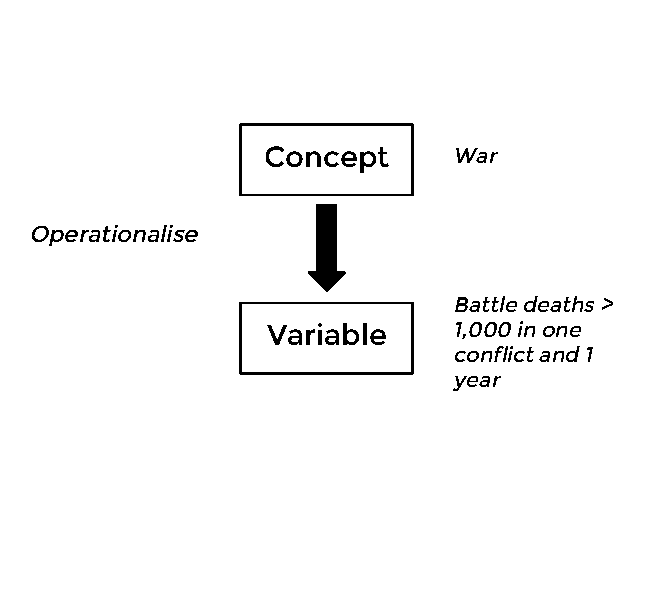
\includegraphics[scale=0.7]{figures/concept_variable.pdf}
    \end{center}
}

\frame{
    \frametitle{When one variable is not enough}

    Frequently in social science we are interested in {\large{complex concepts that cannot be operationalised with one variable}}.

    \vspace{0.5cm}

    Instead, they likely involve {\large{some combination of variables}}.

}

\frame{
    \frametitle{What is it?}

    \begin{center}
        For example, what is democracy?
    \end{center}

}



\frame{
    \frametitle{Why care?}

    \begin{center}
        {\large{Why should we care about measuring concepts well?}}
    \end{center}
}

\frame{
    \frametitle{Why care?}

    \begin{center}
        If we don't have good measures of our concepts, {\large{we can't know how one thing effects another (relationships \emph{between} concepts) and how to improve the social world}}.
    \end{center}
}

\section{Defining the construct}


\section{What data to include}


\section{Normalise variables}

\frame{
    \frametitle{On a level playing field}

    Observable variables are often on {\large{\textbf{different scales}}}.

    \vspace{0.5cm}

    For example, \emph{life expectancy at birth} is in years ranging from 0 to $>100$ and \emph{GNI per capita} is in US dollars starting from $>300$.

    \vspace{0.5cm}

    Obviously, adding these two variables together would {\large{\textbf{weight GNI more than life expectancy}}}.
}

\section{Weighting variables}

\frame{
    \frametitle{Why weight?}

    Once you have your normalised variables ($I_{c,t}$), then you need to consider how to {\large{\textbf{combine}}} them.

    Things to consider:

    \begin{itemize}
        \item {\large{\textbf{Weighting}}}: how important are each individual variables to the composite?

        \item What {\large{\textbf{scale}}} do you want the indicator to be on?
    \end{itemize}
}

\frame{
    \frametitle{Equal weighting}

    If you simply {\large{\textbf{add all of the variables}}} together, you are implicitly assuming that they have an {\large{\textbf{equal weight}}} of {\large{\textbf{1}}}.

    \begin{equation}
        CI_{c,t} = \sum I_{c,t}*1
    \end{equation}

    Sometimes this makes sense: e.g. economic activity is often measured in the same currency.

}

\frame{
    \frametitle{Unequal weighting}


}

\frame{
    \frametitle{Thresholds}

    Sometimes the concept we are measuring might be discrete. E.g. you are in a financial crisis or not in a financial crisis.

    \vspace{0.5cm}

    So, you might set a {\LARGE{threshold}}, a point past which a unit goes from having the characteristic to not having the characteristics.

}

\frame{
    \frametitle{Threshold example}

    Laeven and Valencia (2013) determine a country has crossed a {\large{financial crisis threshold}} if:

    \begin{itemize}
        \item There is `signficant distress' in a country's financial system.

            \begin{center}
                \emph{and}
            \end{center}

        \item At least three of six policy responses are used (e.g. bank holidays, bank nationalisations).
    \end{itemize}
}

\frame{
    \frametitle{Laeven \& Valencia Banking Crises (1970-2011)}

    \begin{center}
        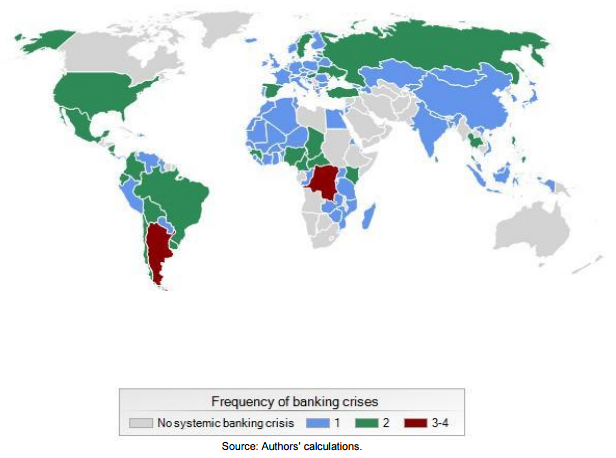
\includegraphics[scale=0.45]{figures/banking_crisis_map.png}
    \end{center}

}

\section{What are we measuring?}

\frame{
    \frametitle{Validity}

    Once you have a composite indicator, your work is {\large{\textbf{far from done}}}.

    \vspace{0.5cm}

    You need to conduct numerous tests to determine if your indicator is a {\large{\textbf{valid}}} measure of the concept you are tying to measure.

}

\section{Pros, Cons, and Pitfalls}

\frame{
    \frametitle{Ranking}

    Composite indicators are popularly used to {\large{\textbf{rank units}}} (e.g. cities, countries)

    [ADD IMAGE]

}

\frame{
    \frametitle{Uncertainty}

    {\large{\textbf{However}}}, we need to remember that our indicators are {\LARGE{\textbf{estimates}}} of what we want to measure.

    \vspace{0.5cm}

    We are {\LARGE{\textbf{uncertain}}} about how well our indicators capture reality.

    \vspace{0.5cm}

    Uncertainty can be {\large{caused}} by at least:

    \begin{itemize}

        \item Error in our construct (i.e. including or omitting important variables)

        \item Measurement error in our raw data $x_{c,t}$

        \item Error in our weighting.

    \end{itemize}

}

\end{document}
